\chapter{Implementierung}
\label{ch:implementierung}

Den Einstieg in das Programm stellt die Datei \Code{main.py} dar.
Hier wird entschieden, ob ein Online- oder Offline-Spiel, wie bereits in den vorherigen Kapiteln beschrieben, gestartet
werden soll.
Die Implementierungen dieser beiden Spielvarianten sollen in diesem Kapitel beschrieben werden, wobei der Fokus auf
die Online-Verbindung gerichtet ist, da es sich hierbei um die Umsetzung der eigentlichen Aufgabenstellung handelt.

\section{Modellierung des Spiels}
\label{sec:modellierung}

Um eine Grundlage zu haben, auf der die Implmentierung aufgebaut werden konnte, wurde zunächst die Modellierung des
Spiels vorgenommen.
Dazu haben wir geschaut, welche Informationen benötigt und vom Server bereitgestellt werden und wie man diese dann
mithilfe eines objektorientierten Ansatzes abbilden kann. \\

Das Ergebnis der Modellierung ist in \Abbildung{fig:klassendiagramm-modell} zu sehen.
Das \Code{Game} hat Zugriff auf die eigenen Eigenschaften, kennt aber auch alle \Code{Player}, die an diesem Spiel
teilnehmen.
Zudem besteht ein \Code{Game} aus einem zweidimensionalen Array aus \Code{Cells}, die das Spielfeld repräsentieren.
In einer \Code{Cell} können sich dann kein, ein oder nach einer Kollision auch mehrere Spieler befinden. \\

\begin{figure}[htb]
\centering
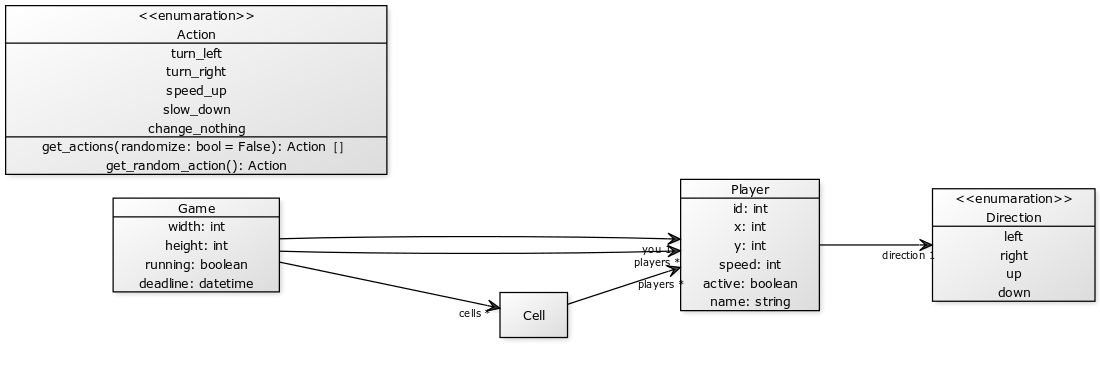
\includegraphics[width=\textwidth]{Bilder/Klassendiagramm_Modellierung.png}
\caption{UML-Klassendiagramm des Modells}
\label{fig:klassendiagramm-modell}
\end{figure}

Da ein Spieler in eine bestimmte Anzahl an Richtungen gedreht sein kann, wird diese Ausrichtung über die Enumeration
\Code{Direction} abgebildet.
Ebenso ist die Auswahl der möglichen Aktionen begrenzt, sodass diese in der Enumeration \Code{Action} festgelegt
worden sind.

\section{Implementierung des Online-Spiels}
\label{sec:online-implementierung}

Um eine Verbindung zu dem \Code{spe\_ed}-Server aufbauen zu können, müssen die URL und ein gültiger API-Key vor dem
Start der Anwendung als Umgebungsvariablen gesetzt worden sein.
Diese Websocket-URL wird entsprechend modifiziert auch als Endpunkt zur Abfrage der Server-Zeit verwendet, auf deren
Nutzung nachfolgend noch eingegangen wird. \\

Die zum Start des Spiels öffentlich bereitgestellte Methode \Code{play()} ist in \Listing{lst:online-play} dargestellt.
Diese ist sehr simpel und ruft lediglich die private Methode \Code{\_\_play()} auf.
Hierbei handelt es sich um eine asynchrone Methode, wie schon in der Methoden-Signatur deutlich wird.
Es wird mittels der Bibliothek \Code{asyncio} sichergestellt, dass diese asynchrone Methode vollständig verarbeitet
wurde, bevor der Kontrollfluss im Programm weiterläuft.
Sobald dies der Fall ist, ist das Spielende eingetreten und die Oberfläche wird beendet. \\

\lstinputlisting[label=lst:online-play,language=Python,caption=\Code{play()}-Methode des \Code{OnlineController}s]
{./Dokumente/OnlineController-play.txt}

In der im vorherigen Absatz bereits erwähnten Methode \Code{\_\_play()} in dem \Code{OnlineController} wird eine
Websocket-Verbindung zum Server aufgebaut.
Anschließend wird in einer Endlosschleife die Logik zur Ausführung eines einzelnen Spielzugs ausgeführt.
Wie ein solcher Spielzug abläuft, ist in \Anhang{fig:sequenzdiagramm-spielzug} in Form eines Sequenzdiagrammes
nachvollziehbar und die Umsetzung im Python-Code kann zusammen mit dem Verbindungsaufbau dem \Anhang{lst:online-__play}
entnommen werden.

\subsection{Einlesen des Spiel-Zustands}
\label{subsec:einlesen-spielzustand}

Der Beginn einer neuen Spielrunde wird damit eingeläutet, dass neue Daten über die Websocket-Verbindung vom Server
versendet werden.
Dabei handelt es sich jeweils um den aktuellen Zustand des Spiels mit allen notwendigen Daten.
Zur Serialisierung wird das Spiel in ein JSON-Format übersetzt.
Ein Beispiel zur Veranschaulichung dieses Formats ist in \Anhang{lst:json-spiel} abgebildet.
Anzumerken ist, dass die exakte Formatierung des Strings abweichen kann. \\

Dieser eingelesene String wird an ein Objekt der Klasse \Code{JSONDataLoader} übergeben, welches die Übersetzung des
JSON-Formats in ein \Code{Game}-Objekt - das wie in \Kapitel{sec:modellierung} beschrieben modelliert ist - zur Aufgabe
hat. \\

Sobald das Spiel fertig aufgebaut wurde, wird ein \Code{GET}-Request an den Server geschickt, auf welchen als Antwort
die aktuelle Server-Zeit erwartet wird und ebenfalls durch den \Code{JSONDataLoader} aus einem String in ein
\Code{datetime}-Objekt geparst wird.
Diese Server-Zeit wird dann verwendet, um durch einen Abgleich mit der Zeit des eigenen Systems gegebenenfalls die
Deadline für die Festlegung auf die nächste Aktion zu verschieben, da diese sich immer nach der Server-Zeit richtet.
Es wird hierbei eine Toleranz von drei Sekunden eingebaut, da je nach Internet-Verbindung die Anfrage an den Server
etwas dauern kann und so die Aktion besser zu früh als zu spät übermittelt werden sollte.

\subsection{Ermittlung der besten Aktion}
\label{subsec:ermitteln-aktion}

Anschließend ist das Spiel in seinem aktuellen Zustand korrekt abgebildet.
Als nächstes steht an, dass eine Entscheidung für die nächste Aktion getroffen werden muss.
Dies ist allerdings nur notwendig, wenn der eigene Spieler noch aktiv ist. \\

Die Berechnung und Festlegung auf die nächste Aktion wird von dem \Code{OnlineController} an ein Objekt einer
Subklasse der abstrakten Basisklasse \Code{ArtificialIntelligence} mit dem Aufruf der Methode
\Code{create\_next\_action(game: Game)} delegiert.
Im ersten Schritt wird von einer vergleichsweise schnellen, aber eher schwächeren \ac{KI} eine Standard-Aktion für den
nächsten Zug berechnet, durch die der Spieler nicht direkt sterben wird.
Erst im Anschluss wird die Berechnung der eigentlich ausgewählten \ac{KI} in einem neuen Prozess gestartet. \\

Hierbei kann die Berechnung länger dauern, als in der Spielrunde an Zeit zur Verfügung steht.
Daher wird dieser Prozess eine Sekunde vor Ablauf der Deadline abgebroche, falls die Berechnung der \ac{KI} noch nicht
beendet ist.
Bei einem Abbrch wird dann die Standard-Aktion an den Server geschickt, andernfalls wird die Berechnung der stärkeren
\ac{KI} verwendet.
Welche Art der im \Kapitel{ch:loesungsansatz} beschriebenen \ac{KI}s gewählt wird, steht dem Anwender grundsätzlich
vollkommen frei.

\subsection{Übergabe der Aktion an die Web-API}
\label{subsec:uebergabe-aktion}

Sobald eine Aktion ausgewählt wurde, muss diese dem Server noch mitgeteilt werden.
In der Dokumentation für die diesjährige Aufgabestellung wurde festgehalten, dass auch hier wieder das JSON-Format
verwendet werden soll.
Daher wird die Aktion an die Klasse \Code{JSONDataWriter} überreicht, die einen String folgender Form erstellt:
\texttt{\{\dq action\dq : \dq speed\_up\dq \}}, welcher dann über die Websocket-Verbindung an der Server gesendet wird.

\section{Implementierung des Offline-Spiels}
\label{sec:offline-implementierung}

Bei der Offline-Version des Spiels ging es darum, lokal die eigenen \ac{KI}s gegeneinander spielen zu lassen und
als menschlicher Spieler gegen die \ac{KI} antreten zu können, ohne eine Verbindung zum spe\_ed-Server herstellen zu
müssen.
Dies ermöglichte uns, lokal zu testen und unsere verschiedenen Lösungsansätzen (siehe \Kapitel{ch:loesungsansatz})
gegeneinander auszuprobieren, um zu beurteilen, welche die beste Strategie ist.
Die Implementierung des Offline-Spiels erfolgte in der Klasse \Code{OfflineController}, die entsprechend der Ober-Klasse
\Code{Controller} die Methode \Code{play()} implementiert. \\

Da wir keine Verbindung zum spe\_ed-Server herstellen, erhalten wir keine Aktualisierung des Spiels.
Auch müssen die errechneten Aktionen der \ac{KI} nicht versendet, sondern lokal verarbeitet werden.
Daher haben wir die Spiellogik in der Klasse \Code{GameService} nachgebildet.
Diese Klasse manipuliert das übergebene Spiel und ist somit der Ersatz zum spe\_ed-Server in der Offline-Variante.
Die Klasse \Code{GameService} muss folglich in der oben genannten Methode \Code{play()} des \Code{OfflineController}s
initialisiert werden.
Dazu müssen zunächst \Code{Player}-Objekte und das entsprechende \Code{Game}-Objekt erzeugt werden, welches dem
\Code{GameService} übergeben wird.
Dieses \Code{Game}-Objekt wird dann im Spielverlauf durch den \Code{GameService} manipuliert.

Zusätzlich werden die \ac{KI}s erzeugt und exklusiv einem Spieler zugeordnet, der sich im Spiel befindet.
Solange das Spiel nun läuft, werden der Reihe nach die nächsten Aktionen der
Spieler/\ac{KI}s abgefragt und an den \Code{GameService} weitergeleitet.

\subsection{Implementierung des GameService}
\label{subsec:game-service}

Bei dem Aufruf des Konstruktors wird dem \Code{GameService} ein \Code{Game}-Objekt übergeben, welches abgespeichert
wird.
Zusätzlich erzeugt der \Code{GameService} eine Instanz der Klasse \Code{Turn}, die einen Spielzug repräsentiert. \\

In einem \Code{Turn}-Objekt ist die aktuelle Nummer des Spielzugs und alle Spieler des Spiels enthalten.
Außerdem wird eine Liste mit den Spielern gepflegt, die in diesem Zug noch eine Aktionen durchführen müssen.
Damit ein Spieler seine Aktion durchführen kann, ruft er die Methode \Code{action(player: Player)} auf.
Das Turn-Objekt prüft dann, ob dieser Spieler bereits eine Aktion gemacht hat und wirft in dem Fall eine
\Code{MultipleActionByPlayerException}, sodass dieser Spieler durch den \Code{GameService} aus dem Spiel ausscheidet.
Sollte der Spieler seine erste Aktion in diesem Zug machen, wird er aus der Liste der Spieler mit den ausstehenden
Aktionen ausgetragen und geprüft ob ein neuer Zug initialisiert werden muss, weil dies die letzte erwartete Aktion
in dieser Spielrunde war. \\

Wenn ein Spieler eine Aktion durchführen möchte, verschickt er in der Offline-Variante keine Nachricht an den spe\_ed-Server,
sondern ruft am \Code{GameService} die Methode \Code{do\_action(player: Player, action: Action)} auf.
Die Methode manipuliert dabei das \Code{Game}-Objekt, sodass dies eine äquivalente Aktualisierung zum Erhalt des Spiels
im JSON-Format durch den spe\_ed-Server ist.

Der grobe Ablauf dieser Methode ist wie nachfolgend beschrieben und kann im Diagramm genauer nachvollzogen werden.
\todo{ggf. ein Diagramm einfügen ... Aktivitätsdiagramm?}
Bei dem \Code{Turn}-Objekt wird die Methode \Code{action(player: Player)} aufgerufen, um zu prüfen ob der Spieler eine
Aktion machen darf und ob ein neuer Spielzug nach dieser Aktion beginnt.
Nachfolgend wird dann die Aktion mit der Methode \Code{get\_and\_visit\_cells(player: Player, action: Action)}
simuliert.
Der Code der Methode befindet sich im \Anhang{lst:get-and-visit-cells}.
Dabei wird der Spieler aktualisiert (x- und y-Koordinate, speed), der die Ausführung der Aktion eingeleitet hat und er
wird im \Code{Game} in die \Code{Cell}s eingetragen, die er durch die Aktion neu besucht hat.
Sollte ein neuer Spielzug durch die Aktion entstanden sein, werden Spieler mit Kollisionen inaktiv geschaltet und
geprüft ob das Spiel beendet ist. \\

Mithilfe dieser Logik des \Code{GameService} können wir Spiele autark durchführen.

Bei der Implementierung der Logik wurde darauf geachtet, dass diese auch bei der Implementierung unserer \ac{KI}s
helfen.
Dadurch konnte der \Code{GameService} in den \ac{KI}s häufig genutzt werden, um beispielsweise Züge vorherzusagen oder
zu prüfen, ob Aktionen zum Verlieren führen.

\section{Bereitstellung einer Oberfläche}
\label{sec:bereitstellung-oberflaeche}

Unabhängig davon, ob ein Spiel online oder offline ausgeführt wird, gibt es die Möglichkeit, den Spielverlauf in zwei
verschiedenen Formen dargestellt zu bekommen.
Zum einen lässt sich das Spiel auf der Konsole darstellen und zum anderen als grafische Oberfläche mittels PyGame.
Beide Dastellungsvarianten implementieren das Interface \Code{View}.

\subsection{View-Interface}
\label{subsec:interface-view}

Das Interface \Code{View} deklariert 3 abstrakte Methoden, die durch die Unterklassen implementiert werden müssen.

Die Methode \Code{update(game: Game)} ist dafür gedacht, dem Benutzer das Spielgeschehen fortlaufend mithilfe des
übergebenen \Code{Game}-Objekts darzustellen, sodass immer der aktuelle Stand des Spiels angezeigt wird.
Mit der Methode \Code{read\_next\_action()} soll die Funktionalität bereitgestellt werden, als menschlicher Spieler
eine Aktion durchführen zu können.
Die dritte Methode \Code{end()} ist dafür gedacht, möglicherweise notwendige Schritte zum Beenden der Oberfläche
auszuführen.

\subsection{Darstellung des Spiels in der Konsole}
\label{subsec:oberflaeche-konsole}

Die Umsetzung der konsolenbasierten View geschieht durch die Klasse \Code{ConsoleView}.
Zur Darstellung des Spiels auf der Konsole haben wir uns für das Package \Code{tabulate} entschieden.
Dadurch war es leicht, strukturierte Tabellen in der Konsole auszugeben, was in der Methode \Code{update(game: Game)}
geschieht.
Durch das Attribut \Code{cells} in dem Objekt eines Spiels haben wir bereits die Belegung der Felder auf dem Spielfeld
durch die \Code{Cell}-Objekte.
Dies wird dann ein ein zweidimensionales Array mit Strings überführt.
Wenn sich kein Spieler auf dem Feld befindet, wird ein leerer String ausgegeben, andernfalls die ID des Spielers.
Die Darstellung kann in \Kapitel{sec:nachstellung-spiel} eingesehen werden.\\

Zur Implementierung der Methode \Code{read\_next\_action()} wurde die Eingabe der Konsole durch die Methode \Code{input}
genutzt und entsprechend der Eingabe wird die passende Aktion zurückgegeben.

\subsection{Nutzung von PyGame als grafische Oberfläche}
\label{subsec:oberflaeche-pygame}

Die grafische Oberfläche wurde in der Klasse \Code{GraphicalView} umgesetzt.
Bei der Darstellung des Spiels haben wir uns für die Nutzung der Bibliothek PyGame entschieden.
Der Grund für die Entscheidung ist die leichte Implementierung eines zweidimensionalen Spiels, wie es das Spiel
spe\_ed ist.
Des Weiteren benötigt PyGame einen geringen Aufwand bei der Initialisierung, um ein Spiel rendern zu können. \\

Zur Darstellung mittels PyGame durch die Methode \Code{update(game: Game)} wird dann in einem initialisiertem Fenster
jeder Bereich in Form von Rechtecken farblich bestimmt und aktualisiert.
Befindet sich kein Spieler auf dem Feld, wird es schwarz gezeichnet und andernfalls entsprechend einer festgelegten
Farbe, die dem Spieler zugeordnet ist, befüllt.
Die Darstellung kann in \Kapitel{sec:nachstellung-spiel} eingesehen werden.
Die Implementierung der Methode befindet sich im \Anhang{lst:pygame_update}. \\

Bei der Implementierung der Methode \Code{read\_next\_action()} für die Eingabe der menschlichen Spieler haben wir die
Keylistener von PyGame genutzt.
In einem Event sind alle zurzeit gedrückten Tasten gespeichert und somit können wir filtern, welche Aktion vom Spieler
gewünscht ist und geben diese zurück. \\

Die Methode \Code{end()} wird in der grafischen Oberfläche dazu genutzt, um das PyGame ordnungsgemäß zu beenden.
Außerdem warten wir zehn Sekunden, sodass die letzte ausgeführte Runde des Spiels nachvollzogen werden kann und die
View nicht sofort geschlossen wird.
